%% intro.tex
%%
%% Copyright 2017 Evandro Coan
%% Copyright 2012-2016 by abnTeX2 group at http://www.abntex.net.br/
%%
%% This work may be distributed and/or modified under the
%% conditions of the LaTeX Project Public License, either version 1.3
%% of this license or (at your option) any later version.
%% The latest version of this license is in
%%   http://www.latex-project.org/lppl.txt
%% and version 1.3 or later is part of all distributions of LaTeX
%% version 2005/12/01 or later.
%%
%% This work has the LPPL maintenance status `maintained'.
%% The Current Maintainer of this work is the Evandro Coan.
%%
%% The last Maintainer of this work was the abnTeX2 team, led
%% by Lauro César Araujo. Further information are available on
%% https://www.abntex.net.br/
%%
%% This work consists of a bunch of files. But originally there ware 3 files
%% which are renamed as follows:
%% Renamed the `abntex2-modelo-include-comandos` to `chapters/chapter_1.tex`
%% Renamed the `abntex2-modelo-trabalho-academico.tex` to `chapters/intro.tex`
%% Renamed the `abntex2-modelo-references.bib` to `aftertext/modelo-ufsc-references.bib`
%%
%% This file was originally the main template file, however this main file was
%% split into several new files, which are respectively drastically changed,
%% except this files which contains most of the main documentation message.
%%

% ------------------------------------------------------------------------
% ------------------------------------------------------------------------
% abnTeX2: Modelo de Trabalho Academico (tese de doutorado, dissertacao de
% mestrado e trabalhos monograficos em geral) em conformidade com
% ABNT NBR 14724:2011: Informacao e documentacao - Trabalhos academicos -
% Apresentacao
% ------------------------------------------------------------------------
% ------------------------------------------------------------------------

% The \phantomsection command is needed to create a link to a place in the document that is not a
% figure, equation, table, section, subsection, chapter, etc.
% https://tex.stackexchange.com/questions/44088/when-do-i-need-to-invoke-phantomsection
% \phantomsection

% https://tex.stackexchange.com/questions/5076/is-it-possible-to-keep-my-translation-together-with-original-text
% \chapter*{Introduction}\label{chap:intro}
% \addcontentsline{toc}{chapter}{Introduction}
% \phantomsection

\phantompart
\chapter*{Introduction}\label{chap:intro}
\addcontentsline{toc}{part}{Introduction}
\markboth{Introduction}{Introduction}

Integer programming stands as a cornerstone in addressing complex decision-making problems, offering a powerful framework for modeling combinatorial optimization problems \cite{wolseyFormulations2020}.
In particular, Mixed Integer Linear Programming (MILP) significance stems from its ability to represent combinatorial optimization tasks with linear objectives and constraints.
Although apparently limiting, the linear requirements allow it to model many problems~\cite{nemhauserScopeIntegerCombinatorial1988} and arbitrarily approximate most problems, e.g., through piecewise-linear approximations of the nonlinearities~\cite{camponogaraModelsAlgorithmsOptimal2015}.
On top of that, due to the linearity of the constraints and objective functions, we have reliable algorithms to solve MILP problems.
In fact, due to the modeling capacity and the robustness of the software solutions, MILP has become the workhorse of combinatorial optimization~\cite{bengioMachineLearningCombinatorial2021}.

Nonetheless, solving instances of MILP problems efficiently remains a formidable challenge, motivating the development of heuristic solutions.
The combinatorial nature of MILP implies that algorithms with optimality guarantees have intractable running times, as the search space expands exponentially with the number of integer variables.
Primal heuristics, which aim to quickly finding high-quality feasible solutions to MILP problems, play a crucial role in enhancing the efficiency of optimization algorithms.
Traditional primal heuristics are often rule-based and designed to exploit structures of a given MILP problem.
As a consequence, they lack adaptability, struggling to generalize across diverse problem instances.
As the landscape of optimization problems continues to evolve, there is a growing need for intelligent and flexible heuristics that can adapt to the intricacies of different MILP instances.

% TODO: add references to "successfully applied to MILP"

Recently, deep learning techniques have been successfully applied to MILP, resulting in effective heuristics~\cite{nairSolvingMixedInteger2021,gasseMachineLearningCombinatorial2022,larsenPredictingTacticalSolutions2022,khalilMIPGNNDataDrivenFramework2022,hanGNNGuidedPredictandSearchFramework2023}.
In contrast to handcrafted heuristics, which rely on expert knowledge to exploit theoretical structures of problem formulations, deep learning-based heuristics identify the hidden patterns of problem instances from data.
This data-driven approach relies on the assumption that problem instances are drawn from underlying distributions and, thus, share characteristics not evident in the mathematical formulation.
Such an assumption often holds for practical situations in which problems must be solved repeatedly, and the parameters that define the instances are random variables with unknown distributions~\cite{bengioMachineLearningCombinatorial2021}.

The research area of deep learning applications to MILP has seen a burst of publications in the past years, as seen in Fig.~\ref{fig:scopus-trend}, with plenty of novel methods being proposed.
The comparisons, however, are still limited, which hinders the effective application of the approaches available in the literature.
In this context, this master’s dissertation aims to contribute to developing learning-based heuristics for MILP problems by evaluating existing techniques in novel applications.
More specifically, this work focuses on deep learning models trained with supervision to predict solutions to MILP problems.

\begin{figure}[h]
    \centering
    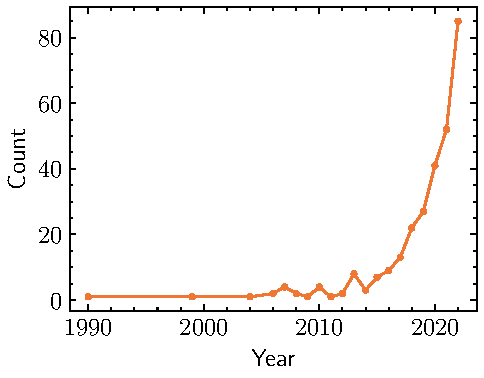
\includegraphics{pictures/scopus.pdf}
    \caption{Number of scientific publications (journal and conference papers) in English language containing the terms "learning" and "MILP" in their title, abstract or keywords. Source: SCOPUS}
    \label{fig:scopus-trend}
\end{figure}

\subsection*{Objectives}\label{chap:objectives}
\addcontentsline{toc}{section}{Objectives}
\markboth{Introduction}{Objectives}

In the topic of this dissertation, three research questions are of fundamental importance in the development of heuristic approaches:
\begin{description}
    \item[Q1] How to design deep learning models to provide candidate solutions for instances of an MILP problem?
    \item[Q2] Which supervised learning techniques are most effective for training solution prediction models for primal heuristics? And
    \item[Q3] How to incorporate solution prediction models in primal heuristics?
\end{description}
Targeting these questions, this dissertation aims \emph{to evaluate primal heuristics for MILP problems based on solution prediction models trained with supervised learning techniques}.
This goal is broken down into three objectives:
\begin{itemize}
    \item Analyze the literature on supervised learning solution prediction models for MILP problems, including model architectures, supervised learning algorithms, and learning-based primal heuristics;
    \item Develop learning-based primal heuristics for a realistic application based on the most promising techniques found in the literature; and
    \item Evaluate the techniques for learning-based heuristics with respect to the empirical performance in a realistic application and the theoretical guarantees provided by each.
\end{itemize}
The achievement of these objectives will result in the two major contributions of this work to the research community.

% \phantompart
